\documentclass{article}
\usepackage{graphicx,tikz}
\usepackage{siunitx,subfig}
\usepackage[graphics,tightpage,active]{preview}
\newcommand{\imsize}{\linewidth}
\newlength\imagewidth
\newlength\imagescale
\begin{document}
\begin{figure}
\begin{preview}
    \renewcommand{\imsize}{\linewidth}
	\centering
	\renewcommand{\imsize}{0.285\linewidth}
	\subfloat[ThreeD]{%
		\pgfmathsetlength{\imagewidth}{\imsize}%
		\pgfmathsetlength{\imagescale}{\imagewidth/596}%
		\def\x{368}% scalebar-x at golden ratio of x=596px
		\def\y{868}% scalebar-y at 90% of height of y=964px
		\begin{tikzpicture}[x=\imagescale,y=-\imagescale]
		\clip (0,0) rectangle (596,964);
			\node[anchor=north west,inner sep=0pt,outer sep=0pt] at (0,0) {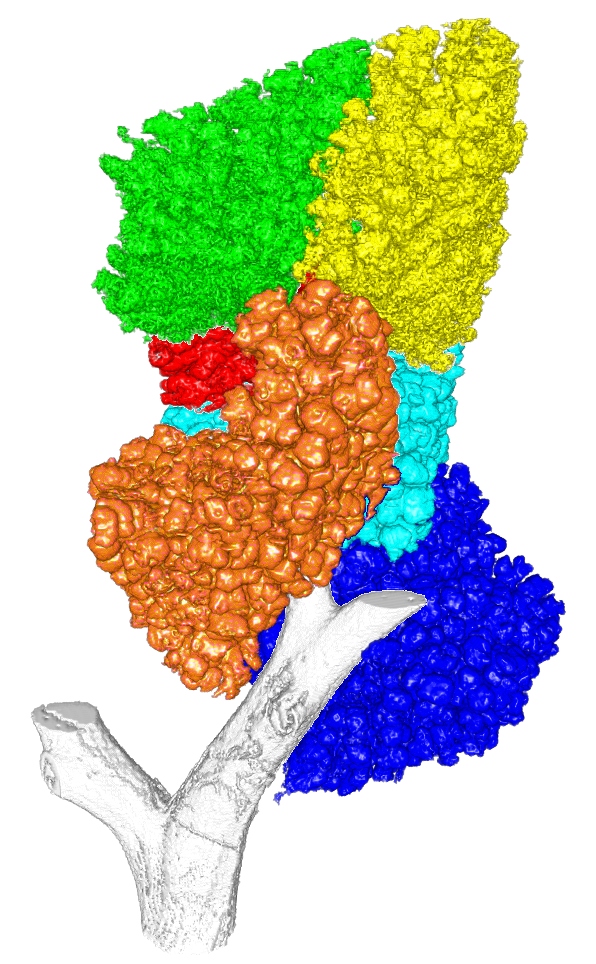
\includegraphics[width=\imagewidth]{AcinarOverlay/R108C04Bt-acini}};
			% 161px = 0.5mm > 100px = 310um > 161px = 500um, 32px = 100um
			%\draw[|-|,thick] (225,395) -- (381,355) node [sloped,midway,above] {\SI{0.5}{\milli\meter} (500px)};
			\draw[|-|,thick] (\x,\y) -- (\x+161,\y) node [midway, above] {\SI{500}{\micro\meter}};
			\draw [red,thick] (65,721) ellipse (50 and 25);
			\draw [red,thick] (49,776) ellipse (25 and 50);
			\draw [red,thick] (262,729) circle (50);
			\draw [red,thick] (392,601) ellipse (50 and 25);
		\end{tikzpicture}%
	}%
	\renewcommand{\imsize}{0.3575\linewidth}%
	\subfloat[Slice 804]{%
		\pgfmathsetlength{\imagewidth}{\imsize}%
		\pgfmathsetlength{\imagescale}{\imagewidth/573}%
		\def\x{57}%was354 scalebar-x at golden ratio of x=573px
		\def\y{660}% scalebar-y at 90% of height of y=733px
		\begin{tikzpicture}[x=\imagescale,y=-\imagescale]
			%\clip (0,0) rectangle (573,733);
			\node[anchor=north west,inner sep=0pt,outer sep=0pt] at (0,0) {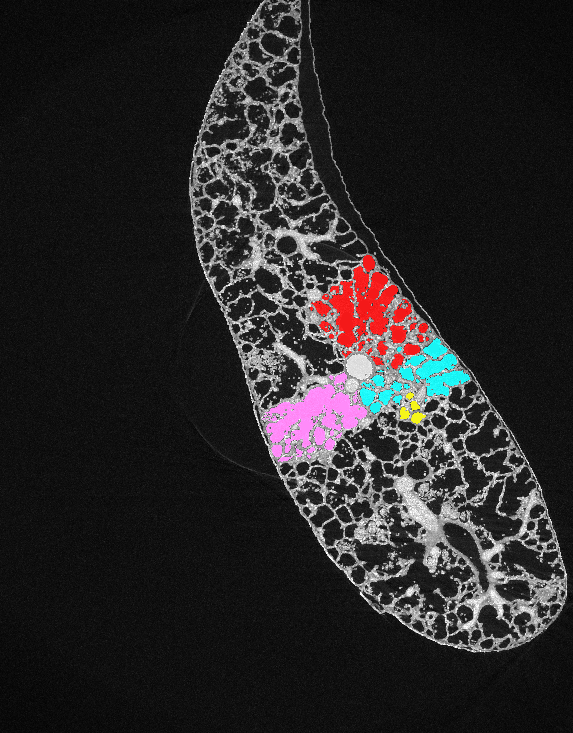
\includegraphics[width=\imagewidth]{AcinarOverlay/R108C04Bt_Slice201_overlay_crop}};
			% 573px = 3.3922mm > 100px = 592um > 84px = 500um, 17px = 100um
			%\draw[white,|-|,thick] (0,128) -- (573,128) node [sloped,midway,above] {\SI{3.3922}{\milli\meter} (573px)};
			\draw[white,|-|,thick] (\x,\y) -- (\x+84,\y) node [right] {\SI{500}{\micro\meter}};
			\draw [white,thick] (286.5,366.5) circle (128);
			\draw [white,thick] (158.5,238.5) rectangle (414.5,494.5);
			\fill [white,nearly transparent] (158.5,238.5) rectangle (414.5,494.5);
		\end{tikzpicture}%
	}%
	\subfloat[Slice 1168]{%
		\pgfmathsetlength{\imagewidth}{\imsize}%
		\pgfmathsetlength{\imagescale}{\imagewidth/573}%
		\def\x{57}%was354 scalebar-x at golden ratio of x=573px
		\def\y{660}% scalebar-y at 90% of height of y=733px
		\begin{tikzpicture}[x=\imagescale,y=-\imagescale]
			%\clip (0,0) rectangle (573,733);
			\node[anchor=north west,inner sep=0pt,outer sep=0pt] at (0,0) {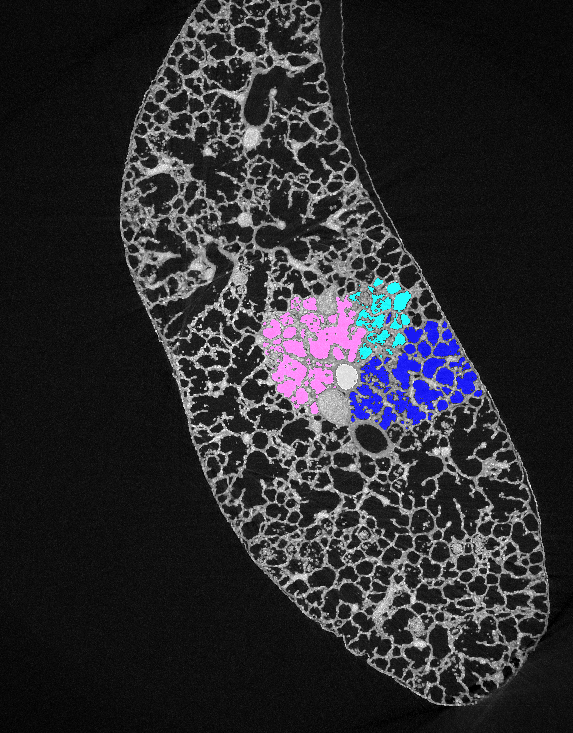
\includegraphics[width=\imagewidth]{AcinarOverlay/R108C04Bt_Slice292_overlay_crop}};
			% 573px = 3.3922mm > 100px = 592um > 84px = 500um, 17px = 100um
			%\draw[white,|-|,thick] (0,128) -- (573,128) node [sloped,midway,above] {\SI{3.3922}{\milli\meter} (573px)};
			\draw[white,|-|,thick] (\x,\y) -- (\x+84,\y) node [right] {\SI{500}{\micro\meter}};
			\draw [white,thick] (286.5,366.5) circle (128);
			\draw [white,thick] (158.5,238.5) rectangle (414.5,494.5);
			\fill [white,nearly transparent] (158.5,238.5) rectangle (414.5,494.5);
		\end{tikzpicture}%
	}%
	\caption{silly caption}%
	\label{fig:acinus overlay}%
\end{preview}
\end{figure}
\end{document}